\uuid{ebva}
\chapitre{Fonction de plusieurs variables}
\niveau{L2}
\module{Analyse}
\sousChapitre{Extremums locaux}
\titre{Un problème d'extrema}
\theme{optimisation}
\auteur{Jean-François Culus}
\datecreate{2024-10-11}
\organisation{AMSCC}
\difficulte{}
\contenu{

\texte{On considère la fonction $f$ définie sur $\R^2$ par 
$$f(x,y)= \left\lbrace \begin{array}{ll}
y^2/x &  ~~~\text{ si } x \neq 0 \\
y & ~~~\text{ si } x=0 
\end{array}\right.$$
}

\begin{enumerate}
\item 
\question{Montrer que $f$ n'est pas continue en $(0,0)$.
}
\reponse{Il est clair que cette fonction n'est pas continue en  $(0;0)$ puisque pour $y$ quelconque fixé, quand $x\to 0$, $f(x,y)\to \pm \infty$.}

\item 
\question{Montrer que $f$ admet des dérivées partielles au point $(0;0)$.}
\reponse{Etudions les dérivées partielles. 
Pour tout $x \in \R^*$, nous avons:
$f(x,0)-f(0,0)=0$ d'où $\lim_{x\to 0} \frac{f(x,0)-f(0,0)}{x}=0$ existe. Ainsi, $\frac{\partial f}{\partial x}(0;0)=0$.
De même pour tout $y\in \R^*$, nous avons:
$f(0,y)-f(0,0)=y$ d'où $\lim_{y\to 0}\frac{f(0,y)-f(0,0)}{y}=1$ et donc la dérivée partielle $\frac{\partial f}{\partial y}(0,0)$ existe est est égale à $1$. 

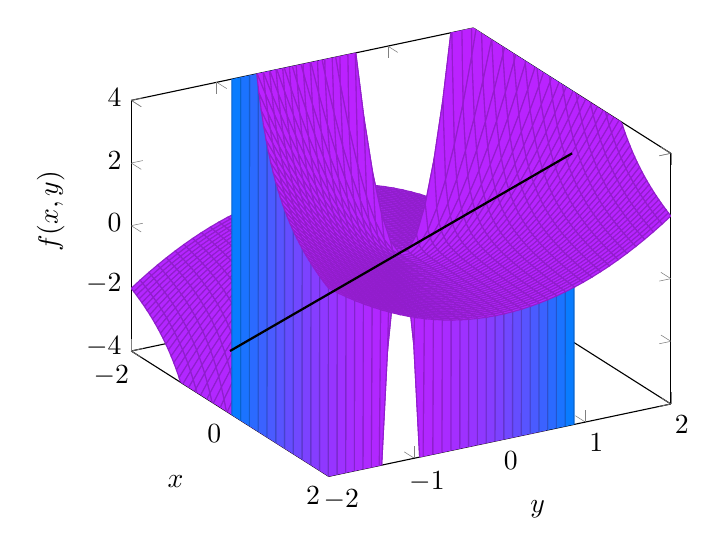
\begin{tikzpicture}
    \begin{axis}[
        view={60}{30},                  % Angle de vue (azimuth, elevation)
        domain=-2:2,                    % Domaine en x
        domain y=-2:2,                  % Domaine en y
        samples=40,                     % Nombre d'échantillons par axe
        xlabel=$x$,                     % Étiquette de l'axe x
        ylabel=$y$,                     % Étiquette de l'axe y
        zlabel={$f(x,y)$},              % Étiquette de l'axe z
        zmax=4,                         % Limite supérieure pour z
        zmin=-4,                        % Limite inférieure pour z
        colormap/cool,                  % Colormap pour les couleurs
    ]
    % Partie pour x ≠ 0 (exclure x=0 pour éviter division par zéro)
    \addplot3[
        surf,                           % Style de tracé en surface
        domain=-2:0.1,                  % Domaine en x (partie négative)
    ]
    {y^2/x};                            % Fonction pour x ≠ 0

    \addplot3[
        surf,                           % Style de tracé en surface
        domain=0.1:2,                   % Domaine en x (partie positive)
    ]
    {y^2/x};                            % Fonction pour x ≠ 0

    % Partie pour x = 0 (cylindre vertical)
    \addplot3[
        domain=-2:2,                    % Domaine en y
        samples=40,                     % Nombre d'échantillons en y
        thick,                          % Épaisseur de la ligne
    ]
    (0,y,y);                            % Fonction pour x = 0
    \end{axis}
\end{tikzpicture}

}
\end{enumerate}
}